\documentclass{standalone}

\usepackage[english]{babel}
\usepackage[linesnumbered, ruled, vlined]{algorithm2e}

\usepackage{caption}

% to create listings

\usepackage{listings, lstautogobble}
\lstset{
  autogobble=true,
  frame=single,
}

\lstdefinelanguage{coq}[Objective]{Caml}{
  morekeywords={Structure, Definition, Inductive, list, return},
  sensitive=true
}

% to create tables, with adaptative column width
\usepackage{array}
\usepackage{tabularx}
\usepackage{adjustbox}
\usepackage{float}

% to define font size

\usepackage{ulem}
\usepackage{moresize}
\usepackage{anyfontsize}

% to use tikz and its libraries

\usepackage{tikz-timing}
\usepackage{tikz}

\usetikzlibrary{backgrounds}
\usetikzlibrary{positioning, calc, arrows, shapes, automata, petri, patterns}

% to use tikzmark, to place and refer to marks outside the current figure

\tikzset{every picture/.style={remember picture}}

% styles for transitions

\tikzset{transition/.append style={fill=black!20, thick}}
\tikzset{transition/.append style={fill=black!20, thick}}

% styles for test and inhib arcs.

\tikzstyle{test}=[pre, *-]
\tikzstyle{inhib}=[pre, o-]

% to use colors

\usepackage{xcolor}

%%%%%%%%%%%%%%%%%%%%%%%%%%%%%%%%%%%%%%%%%%%%%%%%%%
%                  BEGIN DOCUMENT                %
%%%%%%%%%%%%%%%%%%%%%%%%%%%%%%%%%%%%%%%%%%%%%%%%%%

\begin{document}

\begin{tikzpicture}[remember picture]

  \node (table) [inner sep=0pt, text centered] {
    \renewcommand{\arraystretch}{1.5}
    \begin{tabular}{>{\centering\arraybackslash}p{5cm}| >{\centering\arraybackslash}p{2cm}}
    
      \multicolumn{2}{l}{\bf Component C1} \\
      \hline
      behavior & interface \\
      
      \begin{tikzpicture}[remember picture]
        \node[place] (p1) {};
        \node (labelp1) at ($(p1)-(1,0)$) {$P_1$}; 
        
        \node[transition] (t1) at ($(p1)-(0,1)$) {} edge[pre] (p1);
        \node (labelt1) at ($(t1)-(1,0)$) {$T_1$}; 
        
        \node[place] (p2) at ($(t1)-(0,1)$) {} edge[pre] (t1);
        \node (labelp2) at ($(p2)-(1,0)$) {$P_2$}; 
        
        \node[transition] (t2) at ($(p2)-(0,1)$) {} edge[pre] (p2);
        \node (labelt2) at ($(t2)-(1,0)$) {$T_2$}; 

        \node (s1) at ($(t2)-(2,0.7)$) [diamond, fill=black, inner sep=0pt, minimum size=2mm] {};
        \node (labels1) at ($(s1)-(0.4,0)$) {$s_1$}; 
        
        \node (s2) at ($(s1)-(0,0.5)$) [diamond, fill=black, inner sep=0pt, minimum size=2mm] {};
        \node (labels2) at ($(s2)-(0.4,0)$) {$s_2$};
        
        \node (s1) at ($(t2)+(2,-0.7)$) [inner sep=0pt, minimum size=2mm] {};
      \end{tikzpicture}
    & 
      \renewcommand{\arraystretch}{3}
      \raisebox{3cm}{
      \begin{tabular}[t]{c}
        \tikz[remember picture]{
        \node[place] (ip1) [label={[below, yshift=-1cm]: $P_{1-c1}$}] {};
        } \\
        \tikz[remember picture]{
        \node[transition] (it1) [label={[below, yshift=-7mm]: $T_{2-c1}$}] {};
        } \\
        \tikz[remember picture]{
        \node[diamond, fill=black, inner sep=0pt, minimum size=2mm,
        label={[below, yshift=-4mm]: $s_{2-c1}$}]
        (is1) {};
        } \\
      \end{tabular}} \\
    \end{tabular}
  };
  
  \draw[rounded corners=.5em] (table.north west) rectangle (table.south east);
  \draw[dotted] (p1) -- (ip1);
  \draw[dotted] (t2) -- (it1);
  \draw[dotted] (s2) -- (is1);
  
  \node (table1) at ($(table)+(10,0)$) [inner sep=0pt, text centered] {
    \renewcommand{\arraystretch}{1.5}
    \begin{tabular}{>{\centering\arraybackslash}p{2cm}| >{\centering\arraybackslash}p{5cm}}
    
      \multicolumn{2}{l}{\bf Component C2} \\
      \hline
      interface & behavior \\
      \renewcommand{\arraystretch}{3}
      \raisebox{3cm}{
      \begin{tabular}[t]{c}
        \tikz[remember picture]{
        \node[place] (ipp1) [label={[below, yshift=-1cm]: $P_{1-c2}$}] {};
        } \\
        \tikz[remember picture]{
        \node[transition] (itp1) [label={[below, yshift=-7mm]: $T_{2-c2}$}] {};
        } \\
        \tikz[remember picture]{
        \node[diamond, fill=black, inner sep=0pt, minimum size=2mm,
        label={[below, yshift=-4mm]: $s_{2-c2}$}]
        (isp1) {};
        } \\
      \end{tabular}}
      &
        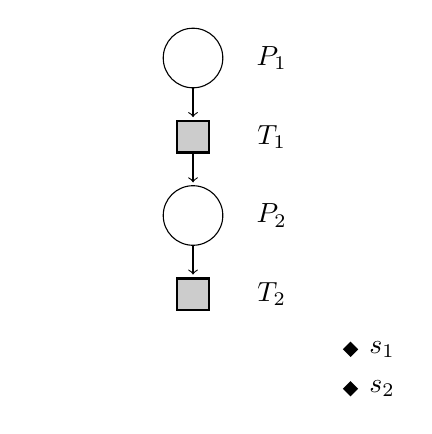
\begin{tikzpicture}[remember picture]
          \node[place] (pp1) {};
          \node (labelpp1) at ($(pp1)+(1,0)$) {$P_1$}; 
          
          \node[transition] (tp1) at ($(pp1)-(0,1)$) {} edge[pre] (pp1);
          \node (labeltp1) at ($(tp1)+(1,0)$) {$T_1$}; 
          
          \node[place] (pp2) at ($(tp1)-(0,1)$) {} edge[pre] (tp1);
          \node (labelpp2) at ($(pp2)+(1,0)$) {$P_2$}; 
          
          \node[transition] (tp2) at ($(pp2)-(0,1)$) {} edge[pre] (pp2);
          \node (labeltp2) at ($(tp2)+(1,0)$) {$T_2$}; 

          \node (sp1) at ($(tp2)+(2,-0.7)$) [diamond, fill=black, inner
          sep=0pt, minimum size=2mm] {};

          \node (labelsp1) at ($(sp1)+(0.4,0)$) {$s_1$};
          
          \node (sp2) at ($(sp1)-(0,0.5)$) [diamond, fill=black, inner
          sep=0pt, minimum size=2mm] {};

          \node (labelsp2) at ($(sp2)+(0.4,0)$) {$s_2$};
          
          \node (sp1) at ($(tp2)-(2,-0.7)$) [inner sep=0pt, minimum
          size=2mm] {};
        \end{tikzpicture} \\
    \end{tabular}
  };

\draw[rounded corners=.5em] (table1.north west) rectangle (table1.south east);
\draw[dotted] (pp1) -- (ipp1);
\draw[dotted] (tp2) -- (itp1);
\draw[dotted] (sp2) -- (isp1);

\draw[dotted] (is1) -- (isp1);
\draw[post] (it1) -- (ipp1);
\draw[post] (itp1) -- (ip1);

\end{tikzpicture}

\end{document}

%%% Local Variables:
%%% mode: latex
%%% TeX-master: t
%%% End:
